\chapter{Introduction}
\label{chp::introduction}

\vspace*{0.5cm}
\section{Motivation}
\label{sec::chp1::motivation}

The \textit{cyberspace} has fuelled the growth of economies and civilisations, but like every innovation, there is a darker side to it; its more ominous aspects are vividly embodied by the idea and existence of the ``dark net.'' The ``cyber'' prefix in words such as cyberspace, cybersecurity, cybercrime, or cyberwarfare has become an element of our everyday lingo. However, it was not too long ago that this reality was considered science fiction. William Gibson coined the term ``cyberspace'' in his 1984 novel \textit{Neuromancer}~\cite{gibson_neuromancer_1984}, describing a virtual and networked grid of data. Our cyberspace is the internet and the World Wide Web, or simply the web; these technologies have become a ubiquitous part of daily life and a key component of national infrastructure. Today, many people in developed economies rely on mobile banking, e-commerce, and digital communication. The internet and the web have become indispensable tools for productivity, communication, and economic growth. However, this growth has also opened new avenues for cybercriminals to exploit vulnerabilities and profit from sensitive user data. Safeguarding user secrets in an increasingly complex and hostile digital environment has become more critical, especially as we conduct more of our sensitive transactions online.

\newpage
We are primarily motivated by countering cybercrime and improving systems that enrich our lives to be more trustworthy and usable. In this dissertation, we focus on distinct steps in the journey of user secrets through cyberspace and devise strategies to circumvent threats. Taking the ``journey of secrets'' perspective differs from similar dissertations \cite{bonneau_guessing_2012, pasquini_enabling_2021, ur_supporting_2016} (primarily password security), and we believe this approach has the added benefit of considering other factors, such as usability and other weaknesses.

\noteBox{\textit{Cyber} and \textit{Cyberspace} Etymology}{%
It is widely believed~\cite{turkle_cyberspace_1999, cohen_cyberspace_2007, benedikt_cyberspace_1994} that ``cyberspace'' was coined by the science fiction writer William Gibson in 1984~\cite{gibson_neuromancer_1984}, which in turn was motivated by the term \textit{cybernetics}. Cybernetics was popularised by Norbert Wiener in 1948~\cite{wiener1948cybernetics}. Cybernetics is a Latin form of the Greek word \textgreek{κυβερνητικός} (kybernetikos), which means ``good at steering''\;---\;a metaphor used to signify the governance of people.
}

\subsection{Cybercrime}
Cybercrime refers to offensive and illegal activities in cyberspace. Examples include fraud, identity theft, data breaches, and data leaks, which can result in significant financial and reputational damage. Cybercrime has a material impact on organisations, individuals, and even nations, leading to economic losses, privacy violations, and national security threats. As cyber threats continue to evolve, understanding their implications becomes increasingly important. We provide some key implications of cybercrime on these entities below.

A \textbf{data breach} refers to unauthorised access to sensitive data, such as credentials and user information, posing a significant threat to individuals and organisations. IBM's \textit{Cost of a Data Breach Report 2023}~\cite{ibm_ibm-2023_2023} indicates that the average cost of a data breach for victim organisations is USD 4.45 million—an increase from the 2020 estimate of USD 3.86 million~\cite{ibm_security_ibm-2020_2020}. 

Beyond the costs of containing the threat and conducting investigations, organisations must also face regulatory penalties. For instance, British Airways was initially issued a £183 million fine, which was later reduced to £20 million~\cite{tidy_british_2020}, for the Man-in-the-Browser (MitB) attack in 2019 (examined in more detail in Chapter~\ref{chp3::breaches}). 

Furthermore, these costs are often transferred to customers through price increases in products and services, as noted in the IBM report~\cite{ibm_ibm-2023_2023}. Users also suffer from potential data leaks, leading to identity theft, account takeovers, and numerous other possible consequences.

Data breaches often lead to \textbf{data leaks}, which then create a vicious cycle of further attacks. Leaked credentials are used for account takeovers or to carry out Credential Stuffing Attacks (CSA) or Credential Tweaking Attacks (CTA). The IBM report~\cite{ibm_ibm-2023_2023} suggests that previously stolen credentials and phishing attacks were responsible for most breaches. Verizon's 2024 Data Breach Investigations Report~\cite{verizon_2024_2024} presents similar findings. Verizon's report indicates that credential misuse through web applications and phishing via email were the most common attack vectors. We build on this analysis by conducting our own empirical investigation of common data breaches in Chapter~\ref{chp3::breaches}.

Organised crime constitutes the majority of \textbf{threat actors}~\cite{verizon_2024_2024}. However, state-sponsored actors exist and are responsible for most sophisticated attacks. While non-state actors are motivated by financial gain, state-sponsored actors are motivated by information gain (spying on other countries) and damaging and weakening their adversaries. For example, the \fun{STUXNET} virus had the aim of slowing down the progress of uranium enrichment in Iran.

Cybercrime has damaging and even paralysing consequences for economies regardless of the actor. Therefore, it is no surprise that governments around the world have created state-funded agencies to counter cybercrime. For example, the UK government's cyber security investment was £1.9 billion between 2016--2021, then increased to £2.6 billion over a three-year period in the 2021 budget review~\cite{uk_cabinet_office_national_2022}. This is reflective of the growing cyber threat that requires further investment at the national level.

\begin{figure}[ht]
    \centering
\noteBox{Case Study: Authentication Scheme Design Requirements}{%
When designing authentication schemes, we must also consider scenarios where users deliberately share their authentication secrets. Here is a case study of such an instance, highlighting how the design of an authentication system can directly impact a company's revenue. Netflix, a subscription-based video-on-demand internet streaming service, has been attempting to address the issue of paying users sharing their credentials with individuals outside their home. This sharing reduces the number of paying customers and thus decreases revenue. Recently, Netflix reported a significant increase in revenue after their password crackdown~\cite{oi_netflix_2024}. In this scenario, Netflix needs to prevent users from sharing their credentials with others.

\vspace*{0.2cm}

Consider when a user $A$ purchases a subscription linked to their identity via an email address $E$ and password $x$, which form their authentication secrets $\langle E, x \rangle_A$. These secrets, of course, can be shared with other users. Note that user $A$ can also have multiple devices themselves. Netflix then limited the number of devices that could stream concurrently. However, this did not solve their primary issue of acquiring more paying users. Let $D_A$ represent a set of devices authenticated with $\langle E, x \rangle_A$. We now need to classify the devices that belong to user $A$ and those that are considered to be \textit{shared}. In this scenario, the authentication becomes $\langle E, x, d \rangle_A$, where $d$ is a vector of device attributes such as IP address, MAC address, device type, etc.
}
\end{figure}

\subsection{Authentication}
\label{sec::chp1::authentication}

Authentication, especially password-based authentication, is a key component of web security, and exploits in these systems are a key threat vector~\cite{verizon_2024_2024}. These systems and protocols serve as the gateway to our identity and secret data online. For these reasons, authentication receives considerable attention in both the literature and industry. Authentication is the act of party $A$ (the \textit{prover} or \textit{claimant}) proving their identity or who they claim to be to party $B$ (the \textit{verifier}). After authentication, the two parties (\textit{principals}) should be assured that they are communicating with each other and not a malicious actor~\cite{burrows_logic_1990}. This is also known as \textit{identification} or \textit{entity authentication}~\cite{menezes_handbook_1997}. In password-based schemes (weak authentication), a username or email address serves as a claim of identity.

Notable related dissertations in the last decade~\cite{bonneau_guessing_2012, pasquini_enabling_2021, ur_supporting_2016} have primarily focused on the guessability of passwords or alternative forms of authentication, such as behavioural biometrics~\cite{drosou_activity_2013} or EEG-based biometrics~\cite{nakamura_wearable_2019}. We take a holistic view by examining the stages of password-based authentication protocols and the journey of other user secrets. This method allows us to capture the weaknesses of the current approach and the limitations of existing research. For example, we find that the literature on password guessing is often disconnected and rarely contributes to the practical security of passwords---we investigate this in Chapter~\ref{chp5::password-guessing-algorithms}.

\subsubsection{Password and the Journey of Secrets}

Passwords are secret strings stored in our memories. They are considered to be a \textit{what you know} form of authentication, which makes them highly usable. If a password is not memorable and is written on a post-it or stored in a password manager, for example, it becomes \textit{what you have}. \textit{What you are} is the last form of authentication. Biometric-based authentication systems are examples of such a form of authentication. The practicality of \textit{what you know} comes at a cost to security, because of the limitations of how much we can remember. Humans also tend to embed predictable patterns in memorable secret strings, which can be exploited to guess them.

Passwords are a weak form of authentication as human-generated secrets are susceptible to being guessed. Passwords encapsulate a paradox where they have to be strong enough to be resistant against being guessed and yet memorable by the user. The user typically generates passwords that are easily guessable. The password distribution exhibits a power law, specifically Zipf's law~\cite{wang_zipfs_2017}. This makes passwords statistically exploitable and computationally feasible to guess. This raises a research question of \textbf{whether a strong password that is human-generated and memorable exists}---we explore this in Chapter~\ref{chp4::password-composition}.

The first line of defence in generating secure passwords is during the composition phase. Tools such as \textbf{Password Strength Meters (PSM)} (such as zxcvbn~\cite{zxcvbn2016}) and \textbf{Password Composition Policies (PCP)} are used to help the user generate stronger passwords, but there is a vast amount of research~\cite{alroomi_measuring_2023, lomchan_comparison_2023, lim_evaluating_2023, maoneke_password_2019, furnell_assessing_2011, woo_survey_2018, lee_password_2022, gerlitz_please_2021, preibusch_password_2010} showing that very few web applications follow any guidance on PCP. Moreover, there is disagreement on the choice of PCP. The choice of PCP is an open problem, which we also explore in Chapter~\ref{chp4::password-composition}.

Passwords are also propped up by other techniques such as \textbf{Multi-factor Authentication (MFA)}. Typically, this is facilitated by SMS, hardware keys, or phone-based OTP. These methods add an extra level of security to mitigate the weaknesses of the password. They, however, can have their own weaknesses too. For example, SMS-based MFA can suffer from SIM swap attacks, which is also a form of identity theft. By impersonating the victim to the telecom provider, the attacker digitally swaps the victim's SIM with their own. This is of course enabled by the fact that organisations still use knowledge about individuals as a form of authentication. Information such as date of birth and address is often enough to conduct identification on the phone. This rudimentary form of authentication is a major contributor to identity theft. The following is a real example of a SIM swap attack: The \$400 million theft of cryptocurrency in 2022 from FTX~\cite{krebs_arrests_2024, belanger_sim-swapping_2024}, known as the ``El Swapo'' attack.

The use of MFA and difficult PCPs comes at a cost to \textbf{usability} and user experience. The use of MFA has of course made password-based schemes more secure, but at a cost to usability and user experience. In many cases, usability trumps security and privacy. The Cookie Policy and regulation was meant to give back rights to the users. The cookie policy pop-ups are a nuisance, so much so that the Brave browser, one that is security and privacy-focused, is blocking them. Users often choose the path of least resistance, and that might not be the most secure path.

The \textbf{storage method} of passwords has a tremendous impact on their security. Storage is the last step in the journey of this secret, and it is a crucial step that directly affects the economy of a guessing attack. Passwords are stored as hash values $y$ using a cryptographic hash function $h$. This function is a one-way function where it takes the input (password) $x$ and creates the hash value output, $h(x) = y$. Typical cryptographic hash functions were designed to be efficient and computationally easy to compute. To deter an attacker from brute-forcing (i.e., computing $h(x) = y$ at speed), we want a function that is resistant to such an attack. These functions are known as \textit{key-derivation functions}. Data breaches often lead to the hash values $y$ being leaked, which are then cracked and revealed to the public. A research question for us is \textbf{whether alternatives to cryptographic hash functions and key-derivation functions exist}. This motivated us to explore zero-knowledge proofs, specifically identity-based cryptosystems in Chapter~\ref{chp::deeid}, which takes us into the password-less authentication territory.

Going beyond passwords is also an active but slow area of research. \textbf{Password-less authentication} is motivated by overcoming the weaknesses of passwords and the usability issues of MFA. The ubiquity of mobile phones and the decrease in the cost of electronics are motivating the use of \textit{what you have} and \textit{what you are} forms of authentication. However, the standards that are being introduced are dogged by confusion and complexity; therefore, the implementation and adoption have been slow. Passkeys were introduced by Apple in 2022. There are privacy concerns in using cloud infrastructure for the storage of cryptographic secret keys. Password-less startups~\cite{wiggers_passwordless_2020, wiggers_passwordless_2023, kovacs_hypr_2022} are being actively invested in. This signals that there is demand for password-less technology.

The above summary of password-based authentication systems and the journey of passwords as secrets reveals many weaknesses that demand a holistic view of security protocols. Perhaps FTX would still be around today had they not lost \$400 million to a SIM swap attack. This dissertation thus takes such an approach. We hope this approach can motivate researchers to be more daring in designing new systems and protocols in a field that is cautious and continuously reminds everyone to stick to what exists and not to innovate.

\subsubsection{Password Guessing Attacks}

It is important to consider guessing methods and algorithms because they help us create stronger passwords and improve password composition policies. Password guessing encapsulates all aspects of a password-based authentication system, where the choice of storage function, the composition of passwords through composition policies, and the appropriate strength meter determine the overall robustness of the password. All these factors influence a password's resistance to being guessed. They receive significant attention in the literature, and with advances in deep learning techniques and architectures, we have seen more guessing methods utilising machine learning. It should be noted that all password guessing research relies on leaked password datasets, and the increase in data breaches has, to some extent, contributed to its growth. Password guessing has also become a ``sport'', as exemplified by the following.

Every year, KoreLogic~\cite{noauthor_korelogic_nodate} hosts a password cracking challenge at the DEFCON\footnote{\href{https://defcon.org}{defcon.org}} conference, and as the premier event of its kind, it attracts the best teams from across the world. Team Hashcat (the developers of the \hashcat password guessing software) have been the winners for the last three years. Their 2023 lineup consisted of 20 hackers, 47 FPGA boards, 78 GPUs, and cloud infrastructure---not your average team. Their post-challenge writeup\footnote{\url{https://github.com/hashcat/team-hashcat/tree/main/CMIYC2023}} provides a strong illustration of how passwords are handled in the real world. Seldom were all the high-performance GPUs running at full capacity because password guessing is more than simply feeding a hash into a machine and waiting for the cleartext output. There are exploitable patterns in these secrets. The KoreLogic challenge mimics this real-world scenario of human-chosen secrets. The goal then becomes discovering the underlying patterns rather than brute-forcing the password. This art is known as \textit{password guessing} in the literature.

\section{Objectives}
\label{sec::chp1::objectives}

We aim to contribute to web security by taking a holistic view of the journey of user secrets. The objectives of this dissertation are as follows:

\begin{enumerate}
\item \textbf{Password Security.} Investigate the weaknesses of the password string through a composition analysis of empirical datasets. Consequently, use this data to compare the different password strength measures and composition policies and provide a recommendation on a usable and secure password composition policy.
\begin{itemize}
\item Create a labelled dataset of passwords showing the composition process of the password. This dataset will contain the password \textit{chunks} and the \textit{transformations}.
\item Propose new methodologies to expedite the password labelling process. Compare the cost and speed of different methods.
\item Investigate how users embed predictable and identifiable information about themselves and their surroundings in their passwords. Identify patterns that have not been clearly identified before.
\end{itemize}

\item \textbf{Server-side Security.} Evaluate the applicability of identity-based cryptosystems in proposed authentication systems in the context of compromised clients or servers.

\item \textbf{Client-side Security.} Propose how the ubiquitousness of mobile phones and cheap micro-boards can be used for the transaction of secrets in the context of a leaky or compromised user device or browser.

\item \textbf{Data Breaches.} Collect and summarise reported data breaches.
\begin{itemize}
    \item Identify the cause of the attacks and categorise each examined report.
    \item Examine the role of authentication systems, especially the role of the password before and after the data breach.
    \item Propose recommendations on how to counter future threats based on the data.
\end{itemize}
\end{enumerate}

\section{Contributions}
\label{chp1::sec::contributions}

We contribute to the field of web security. By taking a novel perspective of the journey of user secrets, we provide an integrated narrative of potential security pitfalls and methods to overcome them. Our contributions are as follows.

\begin{itemize}
%[itemsep=0pt, parsep=0pt]
\item \textit{Breached data:} Using news reports from open-source media outlets, we analysed 60 web security and data breaches that occurred in 2020. We gathered the cause, date, amount and type (PII, finance, health, etc.) of data released, and other information such as fines and the actors behind the attack.
  
\item \textit{Lessons identified and opportunities:} Using the breached dataset, we identified a set of lessons-to-be-learnt and research opportunities. We believe our contributions will be valuable to industry professionals and the research community.
\end{itemize}

\paragraph{Password Security.} Human-generated and memorable secrets, passwords, are crucial a crucial web security components. We contribute to the security of passwords by analysing decades of research, providing new datasets, providing a method to compare password composition policies and consequently recommend the strongest and most usable password composition policy. 

\begin{itemize}
\item \textit{Human-labelled password corpus:} We decompose and label the \hmail-2009~\cite{miessler_hotmail_2009} password strings (8\,292) into chunks, words, structure, tags, and transformations, where applicable. Using the the methods developed in Chapter~\ref{chp4::password-composition}, we machine label the Lizard-Squad 2015 dataset~\cite{miessler_lizardsquad_2015}. To our knowledge, this is the first dataset of its kind. Insights derived from our labelled dataset are discussed, and the dataset is made available for research. This dataset in itself is a novel contribution, we go on to show how it can be used to improve our knowledge of password composition policy.

\item \textit{Password composition:} Utilising our labelled dataset, we evaluate secure and practical password composition strategies. We find that password structures, such as three-word passphrases without semantic links between words, offer both security and practicality. Using the \hmail-2009 dataset and the Lizard-Squad 2015 dataset offers an opportunity to investigate changes in password composition with respect to dates and thus reflect on the age of these datasets. 

\item \textit{Large Language Models and human labellers:} Labelling data is time-consuming and costly, prompting exploration of alternatives to expedite the process. We engaged freelancers from Fiverr~\cite{fiverr2024} and assessed their work against Large Language Models in terms of accuracy, cost, and time. The preliminary results indicate that language models are a promising tool for further experimentation.

\item \textit{Password guessing algorithms.} We provide the first ever systematic exposition of password guessing methods and algorithms. Our aim is to unify the scattered body of knowledge and the disconnect between academic and industry methods in order to create a more rigid and reproducible future experiments.

\end{itemize}

\paragraph{Server-side Security.}
\begin{itemize}
\item \textit{Fiat--Shamir cryptosystem extension:} We propose a new approach to the Fiat--Shamir cryptosystem where an ecosystem can have multiple identity issuers. The cryptosystem is explained in with its design into \deeid in Chapter~\ref{chp::deeid}.
  
\item \textit{Design and implementation of \deeid:} The proposed system is a mobile phone and blockchain-based authentication and identification scheme. We design the system with the Fiat--Shamir identification scheme that utilises a blockchain network as a decentralised PKI. Design of \deeid is explained in Chapter~\ref{chp::deeid}. The implementation constitutes of the following components: mobile phone application, Ethereum smart-contracts, web application and accompanying code. 

\item \textit{Mobile phone and blockchain based authentication scheme:} We compare this new class of authentication scheme through \deeid using the Semi-structured Evaluation of User Authentication Schemes Framework~\cite{bonneau_quest_2012}.

\end{itemize}

\paragraph{Client-side Security.} In Chapter~\ref{chp3::breaches} we find the devastating effect of Man-in-the-Browser (MitB) malware, exemplified by the British Airways case in 2019~\cite{klijnsma_british_2018}. So, our contribution here is a novel out-of-band method to protect user secrets from this malware whilst increasing usability at the same time.

\begin{itemize}
\item \textit{Design and implementation of \formless:} An out-of-band form and data transmission system. Implementation of the proposed system that can circumvent untrustworthy browsers and systems with respect to sending sensitive information to a trusted web server.

\item \textit{Standardising form requests:} We introduce a messaging standard that currently supports payment and sensitive information. Other type of information can be requested by signing the message's \texttt{form\_type} as \texttt{custom}.
\end{itemize}

\section{Dissertation Outline}

\begin{figure}
\centering
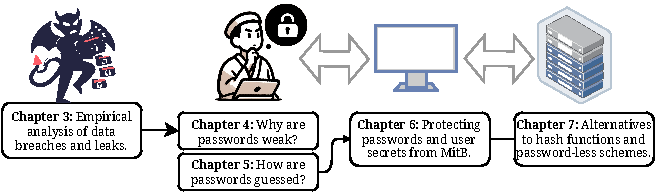
\includegraphics[scale=1.5]{figs/_intro_model.pdf}
\caption{Graphical representation of the dissertation's outline. We explore the journey that user secrets take from the moment a user composes a password to their storage in the server.}
\label{fig::chp1::thesis-outline}
\end{figure}

Figure~\ref{fig::chp1::thesis-outline} presents a graphical representation of this dissertation's structure. To establish a foundation for the dissertation, we conduct our own empirical research on data breaches, which informs the subsequent chapters. The dissertation then explores key checkpoints in the journey of user secrets. The outline of the dissertation is as follows.
\begin{itemize}
\item \textbf{Chapter 2} provides background information and a literature review on authentication schemes, topics related to password security, identity-based cryptosystems, and an overview of common threats to user secrets on both the client and server side. Given the extensive scope of this dissertation, we will include essential background information in the respective chapters when necessary. The majority of the password guessing background and literature will be covered in Chapter~\ref{chp5::password-guessing-algorithms}.
\item \textbf{Chapter 3} investigates the underlying causes of major data breaches. We attempt to validate the findings of IBM~\cite{ibm_security_ibm-2020_2020, ibm_ibm-2023_2023} and Verizon's reports on data breaches using publicly available data. The findings from this chapter will guide the rest of the dissertation. For instance, we chose to conduct an experiment (Chapter~\ref{chp::formless}) on Man-in-the-Browser (MitB) malware due to the high number of reported breaches attributed to this type of attack.
\item \textbf{Chapter 4} aims to address the question of how to compose secure passwords. In doing so, we re-examine why passwords are guessable using the first human-labelled password dataset. We use the data to compare different Password Composition Policies and assess their validity. We find that there is a lack of consensus on what constitutes a strong password, and very few web applications adhere to password guidelines. Using empirical analysis and a novel mathematical framework, we recommend a five-word PCP.
\item \textbf{Chapter 5} continues the discussion on memorable secrets and aims to understand how they are guessed. We provide the first systematic exposition of password guessing methods and algorithms. Our goal is to unify the scattered body of knowledge and bridge the gap between academic and industry methods to create a more rigorous and reproducible framework for future experiments. In this chapter we also produce a framework that uses both quality of generated guesses and the speed at which they are generated. Understanding how passwords are guessed helps us create more robust password composition policies and password strength meters.
\item \textbf{Chapter 6} investigates methods of secret storage on a server. We argue for the adoption of identity-based cryptosystems as a means of overcoming the limitations of cryptographic hash and key-derivation functions when storing memorable secrets. We also demonstrate how Blockchain technology can be used to create identity systems at the national level.
\item \textbf{Chapter 7} evaluates the threats originating from the client-side, specifically the browser. Motivated by the findings in Chapter~\ref{chp3::breaches}, we design and implement a method of circumventing Man-in-the-Browser malware using out-of-band devices. We also incorporate the work from Chapter~\ref{chp::deeid}, using the Blockchain infrastructure to perform identification between the server and the user's out-of-band device.
\item \textbf{Chapter 8} provides a summary and conclusion of the dissertation. We also discuss the ethical issues, applications, and potential economic impact of this research. Lastly, we briefly discuss the personal journey and other work that was experimented with but not included in the dissertation.
\end{itemize}

\section{Publications and Statement of Originality}

I declare that this dissertation was composed by myself, and that the work it
presents is my own, except where otherwise stated. The following
publications arose from work conducted during the course of this PhD:

\begin{itemize}
    \item S.\;Almasi and W.J.\;Knottenbelt. \textbf{Five Word Password Composition Policy}. NDSS Workshop on Measurements, Attacks, and Defenses for the Web (MADWeb 2025), San Diego, California, USA, Feb 2025.
    
    \item S.\;Almasi and W.J.\;Knottenbelt. \textbf{Protecting Users from Compromised Browsers and Form Grabbers.} NDSS Workshop on Measurements, Attacks, and Defenses for the Web (MADWeb 2020), San Diego, California, USA, Feb 2020.
\end{itemize}

Other related work:

\begin{itemize}
    \item S. Almasi and W.J. Knottenbelt. Understanding Password Composition and Strength through Human-labelled and Real Password Datasets. 2024.
    
    \item S. Almasi and W.J. Knottenbelt. Security First API Modelling Techniques. 2021
    
    \item S. Almasi and W.J. Knottenbelt. Research Opportunities and Lessons Identified from Recent Web Security Attacks. 2021
    
    \item S. Almasi and W.J. Knottenbelt. Human Identity and the Quest to Replace Password Continued. 2019
\end{itemize}